\section{Max Słota}
\label{sec:slotamax}

You can see a picture of my spotted catfish below (see Figure~\ref{fig:fish}).

\begin{figure}[htbp]
    \centering
    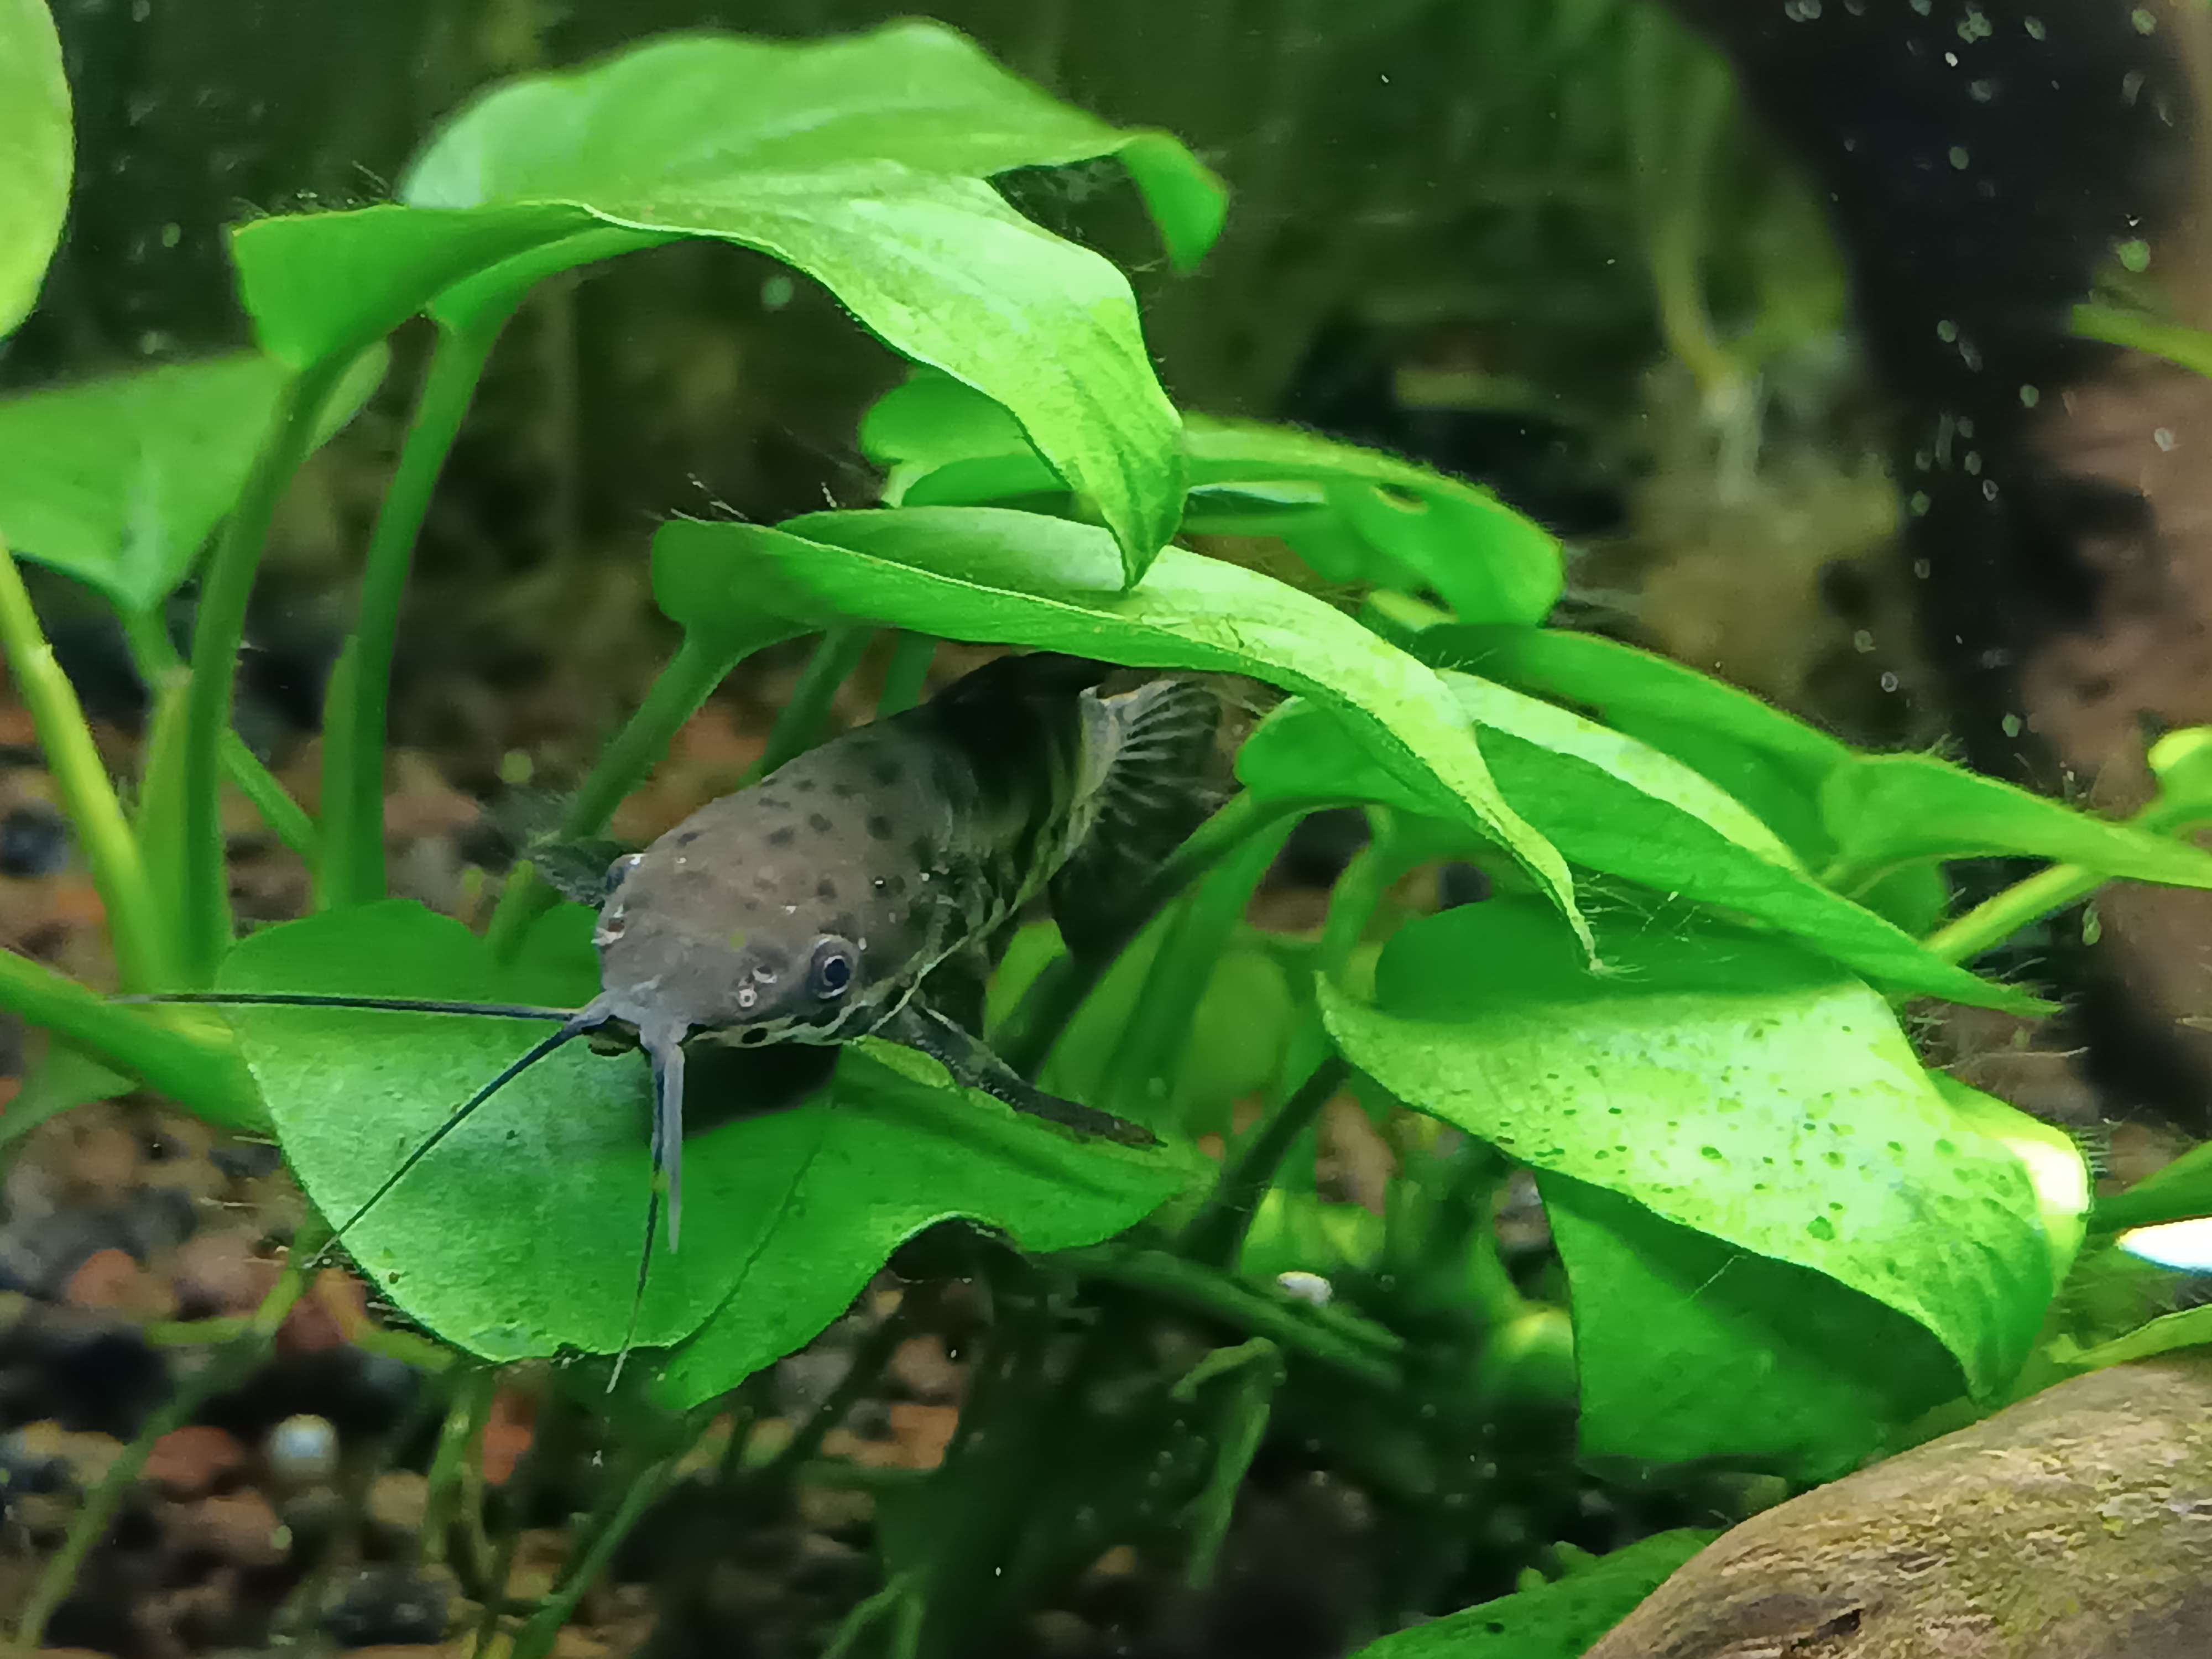
\includegraphics[width=0.5\textwidth]{pictures/fish.jpg}
    \caption{My spotted catfish.}
    \label{fig:fish}
\end{figure}

Table~\ref{tab:multiplication} shows the multiplication of numbers between 1 and 5.
\begin{table}[htbp]
    \centering
    \begin{tabular}{c||c|c|c|c|c}
          & 1 & 2 & 3 & 4 & 5 \\
        \hline\hline
        1 & 1 & 2 & 3 & 4 & 5 \\
        \hline
        2 & 2 & 4 & 6 & 8 & 10 \\
        \hline
        3 & 3 & 6 & 9 & 12 & 15 \\
        \hline
        4 & 4 & 8 & 12 & 16 & 20 \\
        \hline
        5 & 5 & 10 & 15 & 20 & 25 \\
        \hline
    \end{tabular}    
    \caption{This is a multiplication table.}
    \label{tab:multiplication}
\end{table}

Here is the quadratic formula: \[x=\frac{-b\pm\sqrt{b^2-4ac}}{2a}\]

It is used to find the roots of equations of the form $y=ax^2+bx+c$.

\newpage
\noindent{Below is a list of my favourite fruit, with the bullet changed to a '+' sign:}
\begin{itemize}
\renewcommand\labelitemi{+}
    \item Grapes
    \item Watermelon
    \item Peach
\end{itemize}

\noindent{\vspace{3mm} If I were to put them in order, it would look like this:}
\begin{enumerate}
    \item Watermelon
    \item Peach
    \item Grapes
\end{enumerate}

\vspace{5mm}\noindent The \textbf{first paragraph} of this short text is not indented. Both of its paragraphs have been justified. This text is \emph{very interesting} and it is \underline{crucial} that everyone reading it realizes that. Here is some more captivating text in this paragraph.

This is the \textbf{second paragraph}. This time there is indentation. Some of this text has been made \textbf{bold}, \textit{italicized}, or \underline{underlined}. In some cases, \textbf{\emph{\underline{all at once}}}. Here is some more captivating text in this paragraph.